% !TEX program = xelatex
\documentclass[UTF8,a4paper,11pt,fontset=none]{ctexart}
\usepackage[left=22mm,right=22mm,top=18mm,bottom=18mm]{geometry}
\usepackage{fontspec}
\usepackage{graphicx}
\usepackage[table]{xcolor}
\usepackage{fancyvrb}
\usepackage{float}
\usepackage{caption}
\usepackage{booktabs}
\usepackage{tabularx}
\usepackage{fancyhdr}
\usepackage{setspace}
\usepackage{needspace}
\usepackage{enumitem}
\usepackage{etoolbox}
\usepackage{hyperref}

\setmainfont{Times New Roman}
\setsansfont{Times New Roman}
\setmonofont{Courier New}[Scale=0.92, RawFeature={-liga,-dlig,-clig}, HyphenChar=None]
\newfontfamily\codefont{Courier New}[Scale=0.92, RawFeature={-liga,-dlig,-clig}, HyphenChar=None]
\setCJKmainfont{Microsoft YaHei}[
  BoldFont=Microsoft YaHei Bold,
  ItalicFont=Microsoft YaHei
]
\setCJKsansfont{Microsoft YaHei}[BoldFont=Microsoft YaHei Bold]
\setCJKmonofont{Microsoft YaHei}
\xeCJKsetup{PunctStyle=kaiming, CJKecglue={}}
\BeforeBeginEnvironment{Verbatim}{\begingroup\xeCJKsetup{PunctStyle=plain}}
\AfterEndEnvironment{Verbatim}{\endgroup}
\setstretch{1.32}

\definecolor{ink}{HTML}{1C1C1C}
\definecolor{muted}{HTML}{666666}
\definecolor{line}{HTML}{B8B8B8}
\definecolor{head}{HTML}{2F2F2F}
\definecolor{codebg}{HTML}{F6F6F6}
\definecolor{rowalt}{HTML}{F4F4F4}

\hypersetup{colorlinks=false,hidelinks}
\pagestyle{fancy}
\fancyhf{}
\fancyfoot[L]{\fontsize{8.5}{10}\selectfont\color{muted}I3DM 项目复现}
\fancyfoot[R]{\fontsize{8.5}{10}\selectfont\color{muted}\thepage}
\renewcommand{\headrulewidth}{0pt}
\setlength{\headheight}{14pt}
\widowpenalty=10000
\clubpenalty=10000
\displaywidowpenalty=10000

\fvset{
  fontsize=\fontsize{8}{10.2}\selectfont,
  formatcom=\codefont,
  baselinestretch=1.05
}

\captionsetup{
  font={small},
  labelfont={bf},
  textfont={color=muted},
  skip=4pt,
  justification=centering
}

\newcommand{\ask}[1]{%
  \par\vspace{5mm}%
  {\noindent\fontsize{13}{18}\selectfont\bfseries #1\par}
  \nobreak\vspace{1.2mm}%
  {\color{ink}\noindent\rule{\linewidth}{0.45pt}\par}
  \nobreak\vspace{2.6mm}%
}
\newcommand{\point}[1]{\par\noindent\textbf{#1}\hspace{0.4em}}
\newcommand{\src}[1]{\par\vspace{0.6mm}\Needspace{14\baselineskip}\noindent{\fontsize{8.5}{11}\selectfont\color{muted}#1}\par}

\begin{document}
\color{ink}

\begin{center}
{\fontsize{18}{24}\selectfont\bfseries I3DM 项目复现}\\[2.2mm]
{\fontsize{11}{14}\selectfont\color{muted}单张 A100 作业}\\[2.8mm]
{\color{ink}\rule{0.28\textwidth}{0.4pt}}
\end{center}

\vspace{1.5mm}
\noindent
我想讲的是 I3DM，网络用的是官方权重，模型结构我没改过。本科生配额就一张 A100、四个核、一次作业四个小时，官方脚本是按作者那边的机器写的，我一开始想着直接交就能跑，结果卡在下载、评测时间和训练显存上。这张图左列是生成，右列是真值。

\begin{figure}[H]
  \centering
  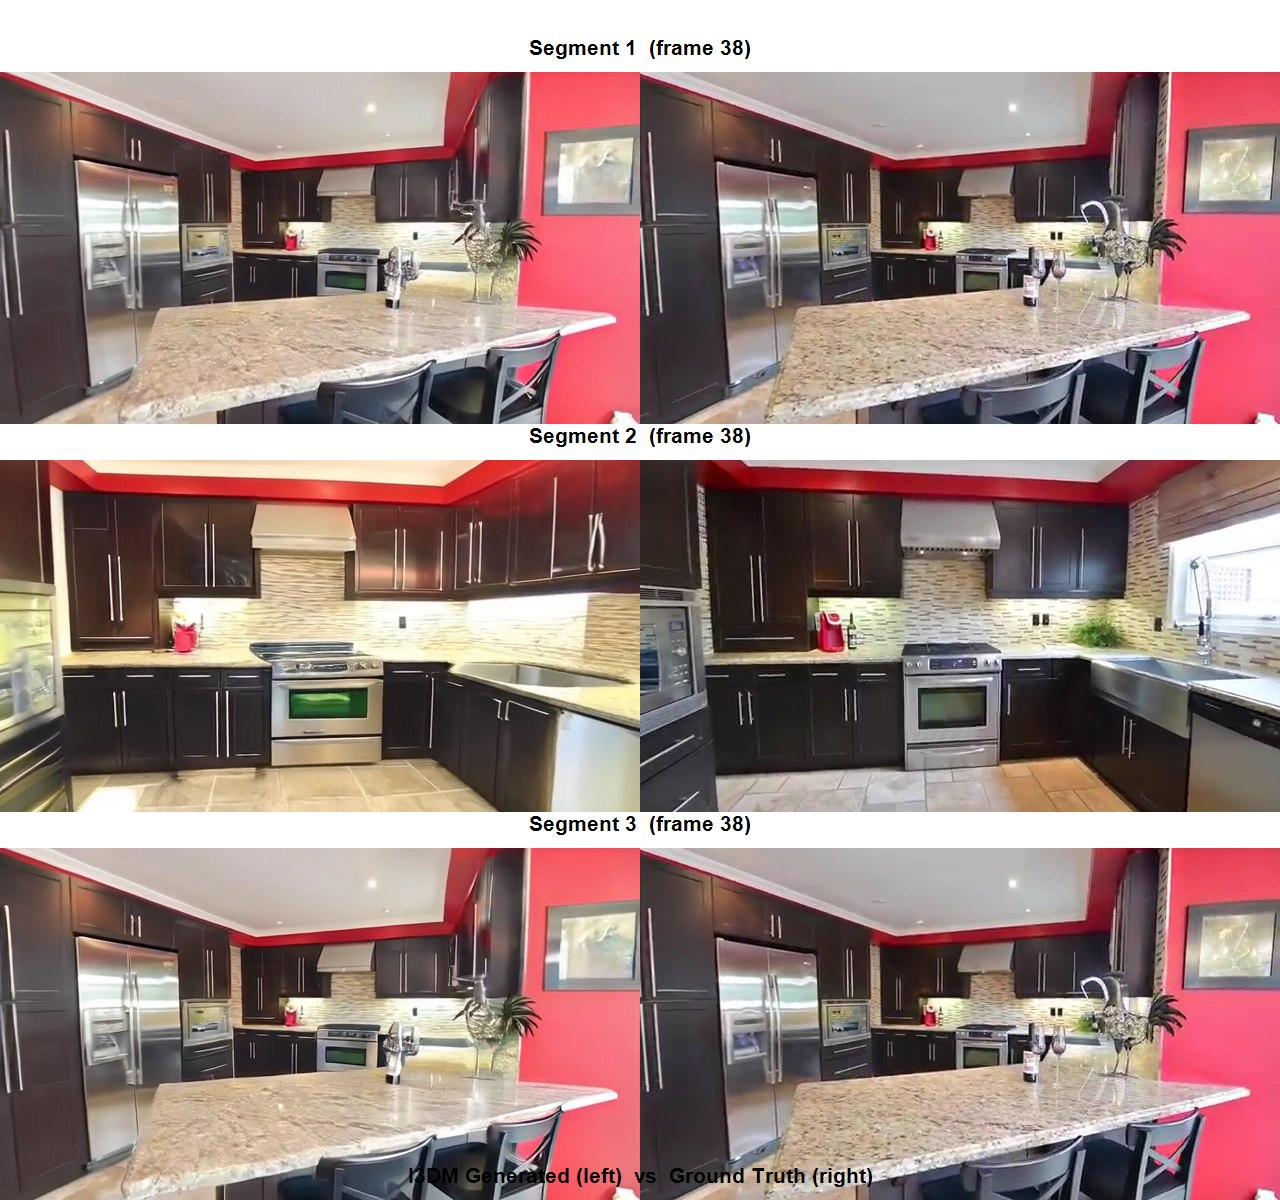
\includegraphics[width=0.72\textwidth]{kitchen_grid.jpg}
  \caption{厨房场景，左列生成，右列真值。}
\end{figure}

\ask{问 1\quad 哪些部分体现了编程能力}

配额卡得死，我一开始还以为调几个参数就行，后来发现很多事得改流程。下面这几段是我实际改过、后来一直在用的。

\point{评测一个场景十来分钟，一次作业装不下。}
我先拿场景 \texttt{8bd3923459d18567} 整段跑通，大约 13 分钟，官方循环里一个场景会按 77 帧切 clip，正向再反向，最后才写成 \texttt{video\_combined.mp4}。按这个速度，4 小时一次只能交十几个——我本来指望一次作业把评测跑完，这下肯定不够。所以跳过放在重置记忆库之前，只认这个合并文件：clip 只出了一半的不算完成，下次整段重跑，免得把半截视频拼进去。场景列表也拆开交，一份大约 16 个，作业脚本把列表当参数传进去，32 个场景的生成和真值都在。

\src{scripts/eval\_re10k.py}
\begin{Verbatim}
print(f"Scene {scene_name} begin generation...")
save_results_dir = os.path.join(base_results_dir, scene_name)
os.makedirs(save_results_dir, exist_ok=True)
if os.path.exists(os.path.join(save_results_dir, 'video_combined.mp4')):
    print(f'==SKIP done== {scene_name}', flush=True)
    continue

mem_bank.reset()
num_clip = (len(test_input_imgs) - ctx_ed) // 76
\end{Verbatim}

\src{eval\_round.sbatch}
\begin{Verbatim}
#SBATCH --gres=gpu:A100:1
#SBATCH -c 4
#SBATCH -t 04:00:00

module load miniconda/py312
source $(conda info --base)/etc/profile.d/conda.sh
conda activate i3dm
cd $HOME/I3DM

LIST=${1:-$HOME/I3DM/data/processed/test/re10k_test_list.txt}
echo "Using list: $LIST"

accelerate launch --num_processes=1 scripts/eval_re10k.py \
  --metadata-path $LIST \
  --output-dir ./results/i3dm_re10K_eval_200
\end{Verbatim}

\point{Re10K 全量是别想了，官方站连不上。}
计算节点访问 \mbox{huggingface.co} 直接不通。一开始我还试着整库拉，结果它把用不到的文件也一起下，纯浪费时间，后来就只挑 index 对得上的下。test 这边下了 121 个，4 小时一次装十几个，接力跑完的是 32 个场景，仓库没有整份克隆。训练另下了一小份，我以为解包就能直接喂进去，结果帧顺序还不保证连续，所以先按文件名里的数字排序，超过 77 帧的按步长切开，尾部不够再留一段盖住结尾，写出新的 json 和列表，251 个场景变成 530 段。改帧之前抽了 200 个样本，核对 \texttt{target\_src\_image} 形状是 77$\times$3$\times$352$\times$640，这次倒是对上了。

\src{scripts/re10K\_clips\_process.py}
\begin{Verbatim}
def frame_sort_key(frame):
    image_path = frame.get("image_path", "")
    stem = os.path.splitext(os.path.basename(image_path))[0]
    try:
        return int(stem)
    except ValueError:
        return stem

frames = sorted(frames, key=frame_sort_key)
start_indices = list(range(0, num_frames, clip_length))
valid_start_indices = [i for i in start_indices if i + clip_length <= num_frames]
if not valid_start_indices or valid_start_indices[-1] + clip_length < num_frames:
    valid_start_indices.append(num_frames - clip_length)
valid_start_indices = sorted(list(set(valid_start_indices)))

for i, start_idx in enumerate(valid_start_indices):
    clip_frames = frames[start_idx:start_idx + clip_length]
    if len(clip_frames) != clip_length:
        continue
    new_filename = f"{base_name}_clip{i}.json"
\end{Verbatim}

\point{作业脚本和环境也得按这台机器改。}
官方 \texttt{requirements.txt} 是他们自己 freeze 出来的，我一开始照着装，有些要编译的包装不上，transformers 太新还会把 torch 往上抬，装到 5 会把 torch 往 2.6 抬。后来锁的是 torch 2.5.0，xformers 跟这个版本走，transformers 停在 4.57.3，模型相关的类能 import，就用这套往下做。平台上还有 5090，这套 torch 跑不了——申请写成 5090 会白等，得写成 A100，还得是大写。sbatch 里路径也得写成绝对路径，进去再 \texttt{module load}、激活 conda，家目录的波浪号在作业里不会展开，这点我后来才注意到。

\ask{问 2\quad 哪些部分体现了 Debug 能力}

问题是一件一件撞上的，同一条训练脚本连续停了好几次，评测也先报过错。我每次先看它停在哪一层，再决定动哪一行——不然容易一上来就改错地方。

\point{缺包不是一次报完，入口文件扫一遍也不够。}
52883 一进来就缺 pandas，补上之后 53053 又缺 easydict，这个倒是写在训练入口顶部。我当时把入口的 import 扫了一遍，觉得齐了，53054 还是挂了，缺的是 wandb。它不在入口那几行里，是 \texttt{WandBModelLogger} 跑起来才 import。装上之后同一次作业才第一次进到前向，后来我知道提交前得把训练用到的 logger 也看一遍，不能只看脚本开头。

\src{scripts/train\_mem\_keyframes\_new.py}
\begin{Verbatim}
from base_diffsynth.trainers.utils import (
    DiffusionTrainingModule, ModelLogger, WandBModelLogger,
    launch_training_task, wan_parser)
from easydict import EasyDict as edict
\end{Verbatim}

\point{前向一跑就 OOM。}
77 帧、640$\times$352，日志里写要 78.5\,GiB，卡是 A100 80GB，就差那么一点，就是装不下。我第一反应是 LoRA 开太大了——rank 1024，怎么想都嫌多。53055 那次就只动了一处当对照：rank 降到 512，帧数碰都不碰，心想显存总该下来一截吧。结果日志还是 78.5\,GiB，几乎没动，我当时还挺意外的，这个方向就放下，不再跟它较劲。现在磁盘上的 \texttt{train\_smoke.sbatch} 是后来留下的，rank 已经写回 1024，\verb|--num_frames| 仍是 77，不是 53055 那一版。

\src{train\_smoke.sbatch}
\begin{Verbatim}
  --lora_rank 1024 \
  --num_frames 77 \
  --height 352 \
  --width 640 \
\end{Verbatim}

显存几乎不动，说明前向吃的不是 rank。我当时有点不信，又去对命令行和实际送进 pipeline 的数。sbatch 写了 77，我一直当它会生效；结果 \texttt{forward\_preprocess} 根本不读这个参数，用的是 \texttt{data["target\_src\_image"].shape[0]}，Dataset 当时 \texttt{num\_target\_views} 还是 77，所以前向一直是 77 帧。降 rank 没把问题修好，但它失败得很干净，只动了一个变量，所以才能把原因收到帧数上。

\src{scripts/train\_mem\_keyframes\_new.py}
\begin{Verbatim}
"input_video": data["target_src_image"],
"num_frames": data["target_src_image"].shape[0],
"height": data["target_src_image"].shape[2],
"width": data["target_src_image"].shape[3],
\end{Verbatim}

帧数只能改在取数据这一层。pipeline 里噪声时间维是 \texttt{(n-1)//4+1}，余数丢掉，所以 \texttt{n-1} 必须能被 4 整除。77 减 1 等于 76，公式上是过得去的，不用它只是显存不够；我中间想过写成 40，一对才发现 39 除不尽，这条是非法的，41 减 1 等于 40，能过。不够长的样本丢掉重抽，rank 加回 1024。53057 用 41 帧跑完 200 步，一步大约 12.6 秒，四个 checkpoint 都写下来了——这回才觉得这件事算过去了。

\src{diffsynth/trainers/unified\_dataset.py}
\begin{Verbatim}
self.num_target_views = 41
self.num_input_views = 4
target_frames = target_data_json["frames"][-self.num_target_views:]
if len(target_frames) < self.num_target_views:
    return self._sample_another()
\end{Verbatim}

\src{diffsynth/pipelines/wan\_video\_mem\_new.py}
\begin{Verbatim}
length = (num_frames - 1) // 4 + 1
shape = (1, pipe.vae.model.z_dim, length, height // pipe.vae.upsampling_factor, width // pipe.vae.upsampling_factor)
\end{Verbatim}

\vspace{1.2mm}
\noindent
\begin{tabularx}{\linewidth}{@{}l>{\raggedright\arraybackslash}X>{\raggedright\arraybackslash}X@{}}
\toprule
\textbf{作业} & \textbf{只改了什么} & \textbf{结果} \\
\midrule
53054 & 补上 wandb，77 帧，rank 1024 & 前向约 78.5\,GiB，OOM \\
53055 & 只把 rank 降到 512 & 显存几乎不动 \\
53057 & 帧数改成 41，rank 回到 1024 & 200 步跑完 \\
\bottomrule
\end{tabularx}

\vspace{1.4mm}
{\noindent\fontsize{9}{12}\selectfont\color{muted}53055 只动了 rank，帧数还是 77，所以显存对得上上一行。}

\begin{figure}[H]
  \centering
  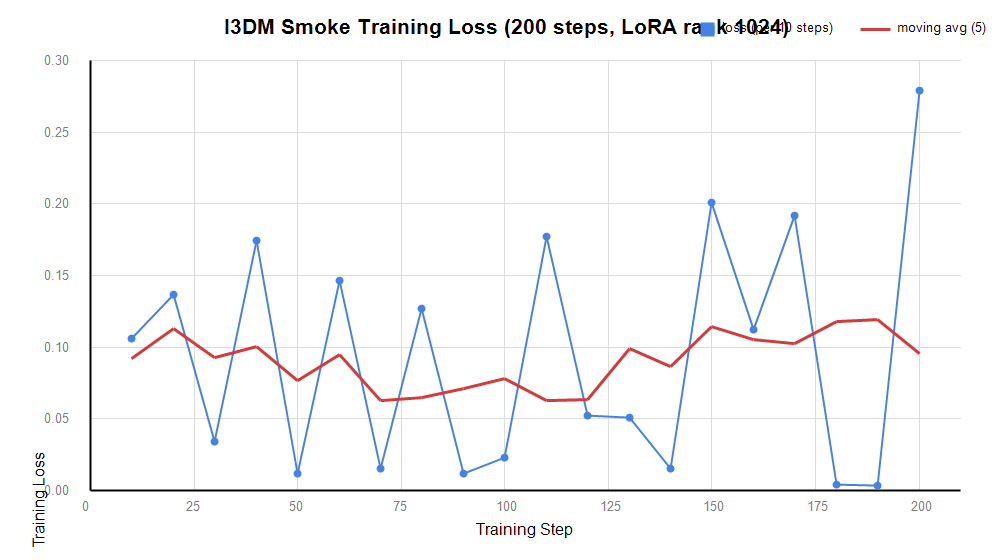
\includegraphics[width=0.68\textwidth]{training_loss_curve.png}
  \caption{200 步 loss 会跳，看着不太顺，但没有 NaN，梯度大约 2.1，权重能写下来。}
\end{figure}

\point{第一次评测报找不到文件，跟显存不是一类问题。}
冒烟评测一上来就说文件不在。数据当时丢在登录节点的 \texttt{/tmp} 里，我在登录节点上 ls 是看得到的，还以为交上去肯定能读，结果交到计算节点就找不到，两边的临时目录不共用。我先在报错的那台机器上确认路径，再把数据挪到家目录，读取代码一行没改，这条就过了。回头看，是我想当然了。

\point{还有一类是卡型和包版本对不上。}
5090、requirements 和波浪号跟问 1 里环境那一节是同一处，我一开始没当回事，被坑过一次之后才都改掉。

\Needspace{12\baselineskip}
\ask{问 3\quad 一般的 debug 思路是怎样的}

报错我一般不急着改。下面这几条都是前面那些作业里用过的。

\begin{enumerate}[leftmargin=1.6em, itemsep=0.55em, parsep=0.15em, topsep=0.4em]
\item 先让它按原样再失败一次，能再复现，我才敢说后面改的是不是这一处。52883 缺 pandas、53053 缺 easydict，都是同一条训练命令再交一次还报同样的错，我才去补包——当时也着急，但改错地方更烦。复现的时候把命令、数据和机器记下来，复现不了，就先对这次和上次差在哪，这个阶段不改刚刚怀疑的那一行。第一次评测就是这样：登录节点上看得到文件，交到计算节点就说没有，差在路径，不在读取代码。

\item 先看现场，再决定假设还成不成立——日志停在哪、实际读到的数是多少，比我第一反应准。sbatch 里写了 \verb|--num_frames 77|，我以为前向就是 77；把 \texttt{target\_src\_image} 的 shape 对上，才知道根本不读这个参数。也先确认跑的是哪份脚本、日志是哪次作业，卡是不是别人还占着。对不上已经看见的现场，这个方向就放下——53055 就是这么放下 LoRA 的。

\item 停在哪一层，就只动那一层，52883 到 53054 都停在 import，这时候改学习率没有意义。评测找不到文件是路径，先看计算节点能不能看见 \texttt{/tmp}；已经跑进前向才崩，才轮到 53054 后面的显存。这三层不放进同一次修改，不然过了也说不清是哪一层好的。

\item 一次只改一个地方，改之前先写下一句预期，要能对上日志。53055 就是这么干的：只把 rank 从 1024 降到 512，帧数不动，心想显存总会下来。结果还是 78.5 左右，所以问题不在 rank，这个改动撤回。后面改 41 帧是另一次，rank 加回去了。好几处一起改，就算过了也分不清是哪一处起的作用，那种「好了但不知道为什么」我不太放心。

\item 说修好了，就用原来触发它的步骤再跑一遍。作业号和日志里的数我会留着，隔一天两次实验不容易混。53057 还是那条训练命令，只是数据变成 41 帧，200 步跑完、权重能写下来，这一处才算过去。小例子过了再把规模加大，加大的时候不再顺手改别的——不然又说不清了。
\end{enumerate}

\end{document}
